% Chapter Template

\chapter{Ensayos y Resultados} % Main chapter title

\label{Chapter4} % Change X to a consecutive number; for referencing this chapter elsewhere, use \ref{ChapterX}

Para la realizacion de los ensayos, comenzamos configurando la PC en forma adecuada. Para ello en la siguiente figura\ref{fig:hw_pc} vamos a ver como configurar en linux la interfaz de red. Es importante destacar que dichos comandos son ejecutados con el permiso se super usuario, \emph{root}.


\begin{figure}[h]
  \centering
  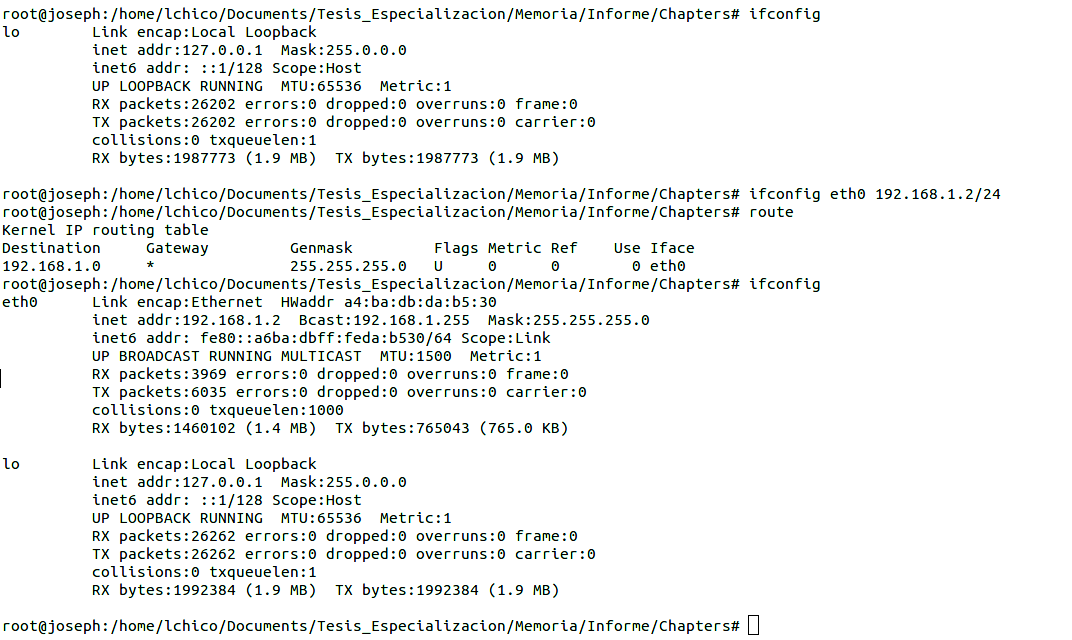
\includegraphics[scale=.35]{./Figures/config_net_console.png}
  \caption{Configuración de una red estatica para la interfaz ethernet.}
  \label{fig:hw_pc}
\end{figure}

Una vez que tenemos la configuracion de red adecuada vamos a proceder a dirigirnos a un navegador web. Y como vemos en la siguiente imagen\ref{fig:web_example} ingresamos el numero de ip correspondiente al dispositivo de control, la cual es: 192.168.1.11 

\begin{figure}[h]
  \centering
  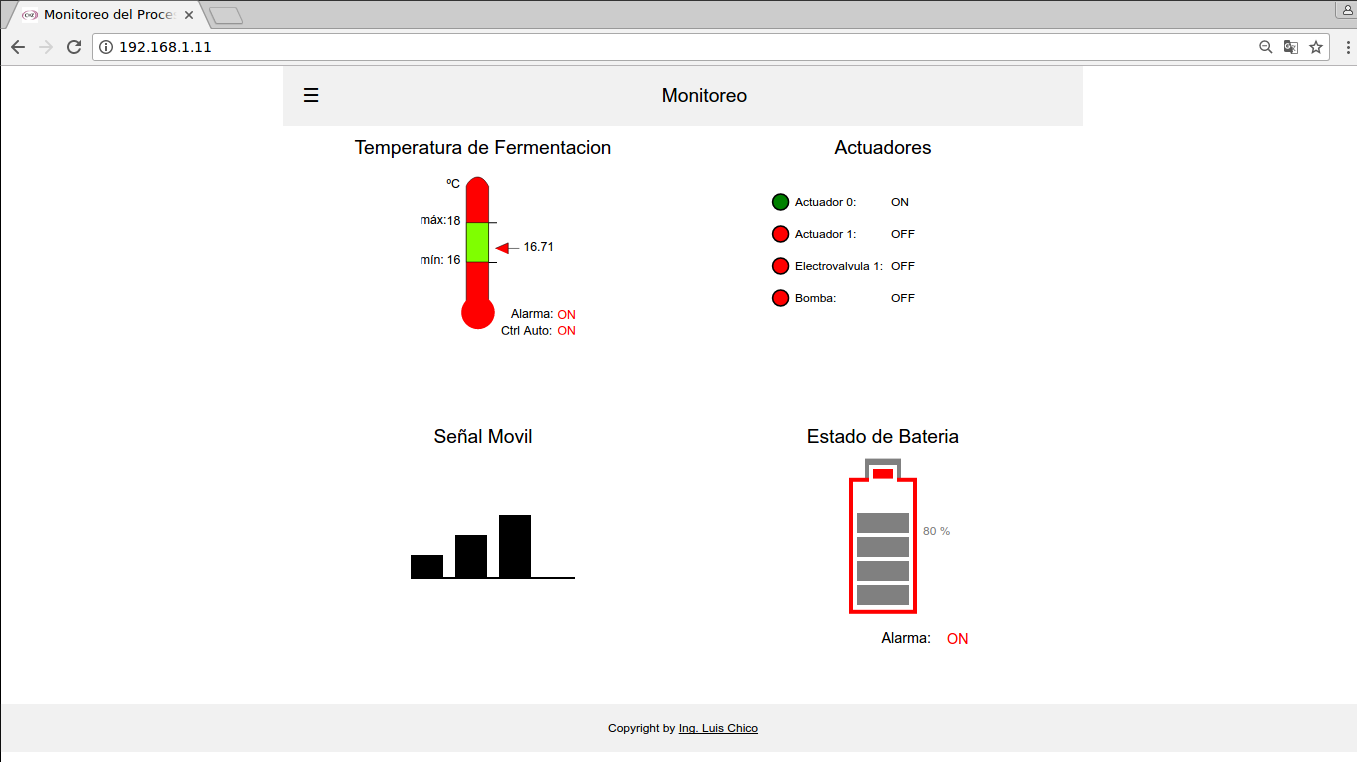
\includegraphics[scale=.25]{./Figures/web_example.png}
  \caption{Pantalla principal de la web de monitoreo.}
  \label{fig:hw_pc}
\end{figure}

En esta pantalla vamos a tener toda la informacion correspondiente al sistema. Arriba a la izquierda podemos ver el estado de la temperatura, con sus rangos maximos y minimos seteados. Y debajo de dicho termometro podemos ver si esta activada: la alarma y el control automatico.

Luego arriba y a la derecha podemos ver los estados de los actuadores, la electrovalvula y la bomba. Estos le permiten al cliente controlar en forma remota dos actuadores y el sistema correspondiente a la bomba de refigeración con la electroválvula asociada. El sensor de temperatura permitira informarle al sistema de control automático cuando debe acutar acorde a los rangos establecidos, esto solo en el caso de estar activado dicho control automático. 

Abajo a la izquierda tenemos en nivel de señal correspondiente al modem GSM, mediante el cual podremos saber si la cobertura de señal de la red de telefonia movil esta en condiciones de operar y permitirnos el servicio de alertas mediante mensajes SMS. 

Finalmente abajo a la derecha tenemos el estado de la batería, el cual va a permitir al sitema continuar en funcionamiento en caso de un corte de energía. El principal uso de este será mantener la posibilidad de enviar un mensaje SMS notificando el corte de energía.




%----------------------------------------------------------------------------------------
%	SECTION 1
%----------------------------------------------------------------------------------------

\section{Pruebas funcionales del hardware}
\label{sec:pruebasHW}

La idea de esta sección es explicar cómo se hicieron los ensayos, qué resultados se obtuvieron y analizarlos.
